\chapter{Introduction}

Current AI systems, such as large language model-based chat-bots and diffusion-based image generators, are primarily trained on fixed datasets.
As a result, they cannot learn from interactions with the world, nor are they designed to engage with their environment in ways that facilitate ongoing learning. 
Similarly, most real-world autonomous systems, such as industrial robots, have to operate within tightly controlled settings so their behavior can be explicitly programmed by human engineers.

% These systems are fundamentally limited by their pre-training data or predefined programming and cannot adapt beyond those constraints.
Developing truly intelligent and autonomous agents capable of acting across diverse and unstructured environments requires us to move past these limitations.
To achieve this, we must enable artificial agents to learn from their interactions with the world in a self-directed manner, using their experiences to improve their capabilities.
This goal has been perhaps most comprehensively pursued within the framework of reinforcement learning \parencite{suttonbook}.

The core idea behind reinforcement learning is that agents are able to improve based on their own experiences.
Each interaction with the world generates a reward signal, which tells the agent how good their current action is.
To improve, an agent seeks to explore the environment to maximize this reward.
This creates the core loop of reinforcement learning: The agent acts in the world, obtains a reward and then seeks to repeat actions that lead to high reward and avoid actions which do not.
Over time, through trial and error, this learning scheme leads to reward-maximizing behavioral policies which an agent can execute to complete the task that is specified by the reward.

The reinforcement learning approach to autonomous agents is a general recipe and has received much attention over the years, with breakthrough successes in playing games \parencite{dqn,silver2016mastering}, robotics \parencite{Hwangbo2019learning,kaufmann2023champion,smith2023demonstrating}, natural language processing and generation \parencite{ouyang2022training,rafailov2023direct,bi2024deepseek}, and industrial applications \parencite{degrave2022magnetic}.
However, despite its broad applicability, reinforcement learning is also often criticized for being unstable, hard to tune, and inefficient \parencite{irpan2018deep,henderson2018deep,patterson2024empirical}.

Many aspects leading to instability and inefficiency have only recently been put into focus.
Recent work has identified culprits such as the failure to properly converge to good solutions \parencite{kumar2021implicit}, lack of generalization and observational overfitting \parencite{song2020observational,kirk2023survey}, and the diminishing ability of agents to learn consistently over many interaction steps \parencite{nikishin2022primacy,hussing2024dissecting}.
All of these reasons lead to a world in which, despite promising results, reinforcement learning has not yet achieved widespread adoption in many domains to which it is ostensibly well suited, such as robotics or scientific research, where discovering new ways of interacting with the complexity of the real world is necessary.


\section{Stable and efficient value function learning}

Can we make reinforcement learning stable and efficient in practice?
To answer this question, we will put our focus on a central problem in reinforcement learning: value function estimation.

The value function is a central concept in reinforcement learning.
Intuitively, it summarizes the expected future return of executing a policy starting from a given state.
Value functions can be used to judge the impact of taking an action, to compare and improve policies, and to guide exploration.
Given their usefulness, a lot of effort has been devoted to obtain good value function learning algorithms, especially using deep neural networks \parencite{dqn,hasselt2010double,hasselt2016deep,fujimoto2018addressing,sac,hussing2024dissecting}.
However, stable and efficient value learning in online scenarios with complex function approximation, such as neural networks, remains an important unsolved problem, and many recent works show persistent problems with existing learning algorithms \parencite{kumar2021implicit,nikishin2022primacy,hussing2024dissecting}.
In this thesis we will show how the problems of the ``deadly triad'' \parencite{suttonbook}, especially bootstrapped value estimation and off-policy data, cause problems with learning stable features in Deep Reinforcement Learning agents.
We present empirical and theoretical investigations into how these instabilities emerge, and propose algorithms to solve these issues.


\subsection{Learning to represent environments}

% To address instability and inefficiency this thesis investigates how agents should represent information about the environment which they gather over the course of training.
% To ensure stable learning, these representations need to be useful for value estimation.
% However, many algorithms struggle with learning such useful representations.

% Learning a value function requires a good representation of the environment.
In order to learn values, an agent needs to filter and process their sensory input and learn about the structure of the environment, the consequences of their actions, and the rewards associated with them.
Most importantly, they need to be able to extract and represent task-relevant information and distinguish it from irrelevant distractions.
In deep learning, we call the output of this process a \emph{representation} of the environment.
This can be any kind of data structure, most often a vector of real-valued numbers, that contains information about the environment and that are useable for machine learning algorithms.
Going back to our initial example, an industrial robot can be tightly controlled and we can pre-specify what it will encounter in its limited environment and how to best represent it for decision making.
But an autonomous agent needs to be able to perceive all of its surroundings and decide, based on current evidence, what information is necessary for its task and how to encode it.
In empirical experiments \parencite{hussing2024dissecting,voelcker2024when,voelcker2022value} we show that failing to do so can lead to unstable value learning.

In supervised learning, neural networks have shown a remarkable ability to extract task-relevant information automatically from raw data, such as images, to solve prediction tasks \parencite{goodfellow2016deep}.
However, in reinforcement learning, this has proven to be more difficult \parencite{jaderberg2017reinforcement,igl2021transient,lyle2021effect,kumar2021implicit,nikishin2022primacy,hussing2024dissecting}.
As the agent explores the environment gradually, it needs to simultaneously learn what information leads to good decisions, and to make good decisions.
This creates a chicken-and-egg problem, as making good decisions requires an agent to be able to represent relevant information, but without knowing how to act, it is unclear what information is relevant \parencite{igl2021transient,voelcker2022value}.
Failing to resolve this problem lead to agents getting stuck in suboptimal policies \parencite{kumar2021implicit,nikishin2022primacy}, or overfitting to irrelevant aspects of the environment \parencite{song2020observational}.

To understand how we can properly represent useful information in reinforcement learning, we will take a close look at two concepts which turn out to be intimately related: environment representations learned by neural networks during training, and world models which predict the behavior of the environment.
Neural network representations are learned functions which map the sensory input of an agent, such as a camera feed or low-level joint information of a robot, to a vector that is useful for reinforcement learning \parencite{ferns2004metrics,jaderberg2017reinforcement,abel2020thesis,le2021metrics}.
World models are functions that allow an agent to explicitly predict how its actions impact the environment.
They can be used to improve value estimation or to plan good action sequences \parencite{dyna,janner2019mbpo,hafner2020dream,schrittwieser2020mastering}.
As we will show, learning a world model provides an excellent way to obtain good representations, and good features simplify learning accurate world models.

\subsection{Balancing decision-awareness and general-purpose learning}
As mentioned, one important problem in representation learning is to be able to separate task-relevant information from distractions.
To properly model task-relevant information, this thesis therefore analyzes \emph{decision-aware} algorithms.
We contrast these with \emph{general-purpose} algorithms, approaches that simply attempt to generate representations and models which can be used for any downstream task.
As we will show, achieving stable and reliable learning requires leveraging and combining both.

\emph{Decision-awareness} describes the idea that the components of a learning approach for decision making, such as representations and models, should account for the final decision task \parencite{vaml,grimm2020value,abachi2020policy,nikishin2021control}.
With this understanding, we can also group many model-free value learning approaches such as DQN \parencite{dqn} or TD3 \parencite{fujimoto2018addressing} under the umbrella of decision-aware methods.
Similarly many supervised learning methods such as classifications are similarly decision-aware as they make use of an explicit task label.

In many cases, representations and world models can also be trained with \emph{general-purpose} methods such as maximum likelihood estimation.
These are unsupervised approaches which seek to simply represent the data through density estimation, compression, or projection.
However, this can be inefficient or suboptimal, as resources are wasted on learning aspects of the data which are irrelevant to the decision-making task \parencite{vaml}.
Instead, a decision-aware algorithm should account for the decision-making task.
In the context of a self-driving car for example, it should put a greater emphasis on certain parts of the observation space, such as a traffic light, instead of others, such as clouds moving in the background of a camera feed.

While this brief introduction seems to suggests that we should always use decision-aware approaches, experimental evidence complicates this conclusion.
Even though decision-aware algorithms promise to be more resource efficient, training with general-purpose methods, for example by fitting a world model with a maximum likelihood objective, often turns out to be more stable in practice \parencite{lovatto2020decision,voelcker2022value}.
In problems such as reinforcement learning, decision-aware algorithms need to continually adapt to the decision task as more information becomes available, and suffer from the aforementioned chicken-and-egg problem.
General-purpose methods on the other hand have a single, stable training objective throughout the learning process.
Especially in the beginning of training when available information about the decision task is limited, using a general-purpose method can lead to a more stable training algorithm.
Therefore, at first glance, efficiency and stability, our two goals, seem to be somewhat at odds with one another.

Addressing this challenge is the contribution of this thesis.
To this end, this thesis puts forth the following hypothesis which guides us through the works presented here:

\begin{quote}
	Effectively combining available information on the decision task with general-purpose learning mechanisms addresses the issues of \emph{instability} and \emph{inefficiency} of value function learning and leads to effective reinforcement learning algorithms.
\end{quote}


\section{Thesis structure}

\begin{wrapfigure}[32]{O}[0pt]{0.4\linewidth}
	\vspace{-2cm}
	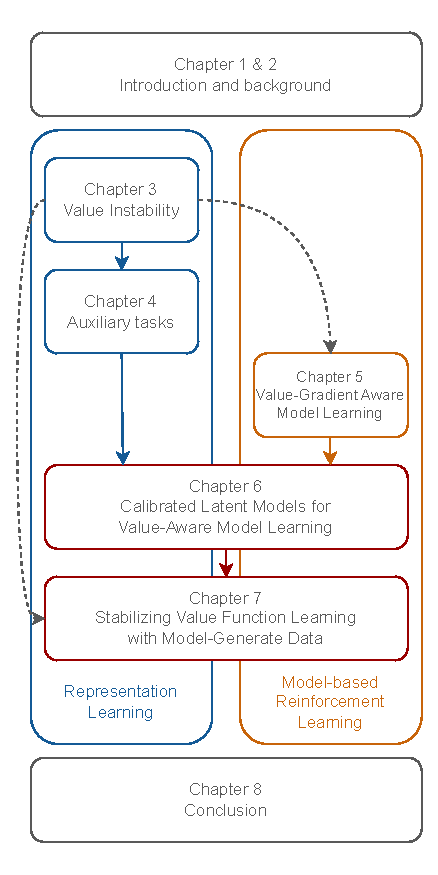
\includegraphics[width=\linewidth]{illustrations/overview_thesis.drawio-1.pdf}
	\caption{An overview of the connections between chapters of the thesis. Chapters 3 and 4 discuss neural network-based representation learning, while Chapter 5 discusses model-based reinforcement learning. Chapters 6 and 7 combine ideas from both strands to establish latent value-aware models with auxiliary task learning. Chapter 3 introduces the problem of learning with high update ratios, which is also used in Chapter 5, and put into central focus again in Chapter 7. Solid lines show influence of algorithmic ideas, and dashed lines mark the problem setting of high update ratio learning.}
	\label{fig:structure_overview}
\end{wrapfigure}

The thesis structure is summarized in \autoref{fig:structure_overview}.
Before diving into the solutions to value learning instability, \autoref{chap:background} presents a thorough overview of important definitions and algorithms in the field of reinforcement learning.
This serves as the background for all further discussions in the thesis.


\autoref{chap:overestimation} presents insights into how instability emerges in value function learning.
Experiments show that one of the major causes of unstable learning is diverging intermediate representations in the neural network architectures.
To address this problem, we introduce an $L2$-norm-based normalization layer into the neural network architecture.
This prevents the feature norm from growing over the course of training and leads to significant increases in learning stability.

\autoref{chap:understanding} dives deeper into the question of stabilizing representations for value function learning.
While several different methods have been proposed in the literature, it remains an open question which model-based auxiliary tasks can be used as general-purpose methods to stabilize learning without deteriorating the quality of the representations for the decision making tasks.
This chapter presents both theoretical and empirical evidence that latent self-prediction models provide beneficial features for this goal.

\autoref{chap:vagram} introduces a second perspective on learning stability and the tension between decision-awareness and general-purpose algorithms by focussing on model-based approaches.
Here we investigate how the instability of value function learning can harm the training of decision-aware environment models.
Empirical evidence is presented that suboptimal value function learning leads to a chicken-and-egg problem: without a good value function, we cannot train a good decision-aware model, but without a good decision-aware model, we cannot improve our value function.
To escape this cycle, we suggest to augment a general purpose MSE loss with a sensitivity score derived from the current value function estimate.
This again highlights how combining both decision-aware and general purpose methods allows us to overcome the challenges of either.

\autoref{chap:cvaml} first shows how previous attempts at decision-aware model learning, including the IterVAML \parencite{itervaml} and MuZero \parencite{schrittwieser2020mastering} losses can be unified into one family. 
We then discuss issues that arise in this framework when using previously established losses naively for learning value functions with stochastic environment models, and show how to mitigate this problem.
The source of the problem is a subtle error term that appears when using the common decision-aware MuZero loss with stochastic models.
Finally, this chapter discusses how latent model architectures, such as those in presented in \autoref{chap:understanding}, can be used to learn strong value-aware models and tame the issues presented in \autoref{chap:vagram}.
With this, we fully unify the ideas of world model and representation learning.

\autoref{chap:mad} presents Model-augmented Data for TD learning (MAD-TD), an empirically strong algorithm that combines the ideas presented in this thesis.
While previous chapters discuss the individual components of MAD-TD, here we put the focus back on solving the issue of instability established in \autoref{chap:overestimation}, tying all of our discussions together.
Using a latent value-aware model with well normalized features addresses a final important problem in value function learning: off-policy generalization.
With a learned model, counterfactual questions of the form ``What would happen if the agent took action $a'$ in a previously visited state $\state$?'' can be answered, which empirically has a strong stabilizing effect on value function learning.

Finally, this thesis concludes with \autoref{chap:conclusion} where we review the findings and discuss remaining questions and promising directions for future work.


